\documentclass[12pt,twoside]{article}
\usepackage{graphicx}
\usepackage{jmlda}
%\NOREVIEWERNOTES
\title
    [Задача поиска смысловых меток в текстах] % Краткое название; не нужно, если полное название влезает в~колонтитул
    {Задача поиска смысловых меток в текстах}
\author
    [Северилов~П.\,А.] % список авторов для колонтитула; не нужен, если основной список влезает в колонтитул
    {Северилов~П.\,А., Лемтюжникова~Д.\,В., Апишев~М.\,А.} % основной список авторов, выводимый в оглавление
    [Северилов~П.\,А.$^1$, Лемтюжникова~Д.\,В.$^1$, Апишев~М.\,А.$^2$] % список авторов, выводимый в заголовок; не нужен, если он не отличается от основного
\thanks
    {
    	%Работа выполнена при финансовой поддержке РФФИ, проект \No\,00-00-00000. Научный руководитель:  
   Задачу поставил:  Лемтюжникова~Д.\,В., 
    Консультант: Апишев~М.\,А.}
\email
    {severilov.pa@phystech.edu, daratigra@icloud.com, great-mel@yandex.ru}
\organization
    {$^1$Московский физико-технический институт (МФТИ); 
    	
	 $^2$Московский государственный университет имени М.В.Ломоносова (МГУ им. М.В.Ломоносова)}
\abstract
    {В работе рассматривается задача поиска смысловых меток в тексте. Определение в тексте средств выразительности таких, как метафоры, аллегории и пр. у экспертов происходит в ручном режиме, и процесс никак не автоматизирован. Эта задача сводится к проблеме Sequence Labeling на размеченной выборке. В работе определяется применимость методов Sequence Labeling к задаче. Тестирование проводится на тексте романа М. А. Булгакова "Мастер и Маргарита" и датасетах с английскими метафорами.

\bigskip
\textbf{Ключевые слова}: \emph {смысловые метки, LSTM, sequence labeling, cкрытые марковские модели}.}
\titleEng
    {JMLDA paper example: file jmlda-example.tex}
\authorEng
    {Author~F.\,S.$^1$, CoAuthor~F.\,S.$^2$, Name~F.\,S.$^2$}
\organizationEng
    {$^1$Organization; $^2$Organization}
\abstractEng
    {This document is an example of paper prepared with \LaTeXe\
    typesetting system and style file \texttt{jmlda.sty}.

    \bigskip
    \textbf{Keywords}: \emph{keyword, keyword, more keywords}.}
\begin{document}
\maketitle
%\linenumbers

\section{Введение}
 Модели для обработки текстов не справляются с главной особенностью языка — неоднозначностью смысла высказывания. Текст воспринимается ими буквально (в прямом смысле), и различные \emph{смысловые метки} не интерпретируются верным образом. 
 %Так, например, выражение «золотые руки» вероятнее всего будет понято моделью, как «руки из золота» вместо верного «умения очень хорошо делать что-либо».

Задача поиска смысловых меток в тексте  в этой работе сведена к sequence labeling -- более общей задаче, широко распространенной в NLP [2]. Рассматриваются три типа sequence labeling: тегирование частей речи (part-of-speech tagging), распознавание именованных сущностей (named entity recognition) и синтаксический анализ (shallow parsing). Данные методы применены к текущей задаче.

 Задачи sequence labeling решаются с использованием линейных статистических моделей [1][3], например: скрытые марковские модели, марковские случайные поля. Реализация решений происходит с помощью различных архитектур нейронных сетей. В данной статье сравниваются результаты работ нескольких моделей нейронных сетей для sequence labeling применительно к задаче поиска смысловых меток. Архитектуры таких сетей -- рекуррентные сети, а именно Bidirectional LSTM с использованием CRF. Рассматривается три подхода [1]. Первый -- это BiLSTM, второй -- модификация: на вход сети подаются не векторные представления слов в целом, а каждый символ по отдельности. Третий подход основан на предыдущей модели, но с интеграцией механизма внимания (attention) в архитектуру. %(Transformer).
%\cite{author09anyscience,myHandbook,author09first-word-of-the-title,voron06latex,author-and-co2007,Lvovsky03}.
\section{Задачи распознавания смысла в тексте}
\subsection{Задача определения смысловых меток}
Пусть $W=\{w_1,\ldots,w_n\}$ --- множество слов, $Z=\{z_1,\ldots,z_p\}$ --- множество значений.

Определение 1. Метками слова $M=\{m_1,\ldots,m_r\}$ будем называть способы интерпретации значения $z$ относительно слова $w$.

Примеры меток: разговорный, эпитет, символ, метафора, ругательный, переносный.

Определение 2. Смыслом слова $w_i$ будем называть тройку элементов $S_{i,j,k}=<w_i, z_j, m_k>$. 

Примеры: <абрикосовый, цвет, эпитет>, <ад, невыносимое положение, гипербола>, <флаг, страна, метонимия>.

%Определение 3. Словарём смыслов будем называть множество смыслов слов $S_{i,j,k}=<w_i, z_j, m_k>, \forall w \in W_S \subset W$.

%Гипотеза 1. Словарь смыслов будем считать неполным, поскольку не существует словарей для всего множества слов языка с описанием всех значений и меток.

Определение 3. Контекстом $k$ будем называть набор слов $\{w_1,\ldots,w_l\}$, где $w_i\in W$. Текстом $T$ будем называть множество контекстов $\{k_1,\ldots, k_q\}$.

Определение 4. Контекстным словарём будем называть четвёрку\\ $Y_{i,j,k,q}=<w_i, z_j, m_k, k_q>$.

Гипотеза 1. Контекстный словарь будем считать неполным, поскольку не существует словарей для всего множества слов языка с описанием всех значений и меток относительно каждого возможного контекста.

Определение 5. Дополнением контекстного словаря будем называть новый словарь $Y^*_{i,j,k,q}$, в котором существует хотя бы один из элементов\\ $<w^*_i, z^*_j, m^*_k, k^*_q> \notin Y$.

Определение 6. Пусть имеются множества слов в двух контекстах \\ $W_{k_1} \in k_1, W_{k_1} \in k_2$. Каждому слову из $W_{k_1}$ и $W_{k_2}$ соответствуют значения $Z_{k_1}$ и $Z_{k_2}$. Уровнем близости контекстов будем называть величину $\psi(k_1, k_2)$, равную совпадающему числу значений слов из данных контекстов\\ $|Z_{k_1}\cap Z_{k_2}|$.

Пример: $k_1=$ <<За последнее десятилетие делаются попытки проникнуть в глубь строения материи, открывающие безграничные возможности будущего ее технического использования>>, $k_2=$ <<Им владели другие творческие интересы, влекли к себе безграничные художественные горизонты живописи>>. $\psi(k_1, k_2)=|Z_{k_1}\cap Z_{k_2}|=\{$ безграничный = имеющий такую большую степень, что он мыслится как не имеющий предела; горизонт = возможность = граница, до которой говорящий представляет себе существование и развитие масштабного явления А1$\}=2.$ 


Определение 7. Пусть даны текст $T$, контекстный словарь $Y$, дополнение контекстного словаря $Y^*$. Задачей определения смысловых меток будем называть нахождение нового дополнения контекстного словаря $Y^{**}$: $\exists w_i \in T: \exists <w_i, z^{**}_j, m^{**}_k, k^{**}_q> \notin Y, Y^*$.  


\subsection{Задача поиска метафор}
При подходе нахождения смысловых меток задача поиска метафор сводится к задаче определения смысловых меток, если метка принимает значение <<метафора>>. Рассмотрим другой подход, основанный на частотности значений слов. Перейдём к литературному определению понятия метафора.

Определение 8. Метафора --- слово или выражение, употребляемое в переносном значении, в основе которого лежит неназванное сравнение предмета с каким--либо другим на основании их общего признака.

Таким образом, чтобы формализовать данное определение, необходимо формализовать понятие признака для двух слов, а также затронуть понятия прямого и переносного значения слова. 

Определение 9. Частотой слова $w$ относительно значения $z$ будем называть величину $\nu(w,z):$
\[
\nu(w,z) = \frac{\sum_{q}|\{<w, z, m_k, k_q>\}|}{\sum_{j}\sum_{q}|\{<w, z_j, m_k, k_q>\}|} \cdot 100\%
\]
Также будем говорить, что слово $w$ в значении $z$ употребляется с частотой $\nu$.


Гипотеза 2. Значения слов с наибольшей частотой употребляются в прямом значении.


Определение 10. Контекстным расстоянием между словами будем называть величину $\rho (w_1, w_2):$

\[\rho (w_1, w_2) =
\begin{cases}
1, \exists k: w_1, w_2 \in k; \\
0, \text{иначе}
\end{cases}
\]
Если $\rho (w_1, w_2)=1$, $w_1$ и $w_2$ --- соседи. Все соседи $w_1$ --- окрестность $w_1$.
Сумму расстояний $\rho (w_1, w_2)$ для всех возможных контекстов будем называть суммарным расстоянием слов $w_1$ и $w_2$. Отношение суммарного расстояния и всего множества контекстов будем называть контекстной частотой слов $w_1$ и $w_2$. 

Определение 11. Фразеологизмами будем называть пару слов, которые имеют высокую контекстную частоту, но при этом употребляются в переносном значении. Множество пар фразеологизмов и их значений будем называть словарём фразеологизмов.

Примеры фразеологизмов: <<кот наплакал>>, <<бить баклуши>>, <<тянуть за язык>>

Замечание 1. Фразеологизмы также относят к одному из видов метафор --- метафоры--формулы. Их характеризует невозможное преобразование в конструкцию, когда значение всего словосочетания можно получить прямым поиском значений каждого слова. 

Гипотеза 3. Слова с высокой контекстной частотой, которые не являются фразеологизмами, употребляются в прямом значении.

Определение 12. 
Признаковым пространством слова будем называть подмножество соседей с наиболее высокой контекстной частотой.

Определение 13. Для соседей $w_1$ и $w_2$ метафорой будем называть слово $w_2$, которое не входит в признаковое пространство $w_1$, но одно из переносных значений слова $w_2$ совпадает с прямым значением слова, которое входит в признаковое пространство $w_1$.

Примеры метафоры. 

%Первый пример метафоры. <<В саду горит костёр рябины красной>>. Словосочетание <<горит костёр>> не входит в признаковое пространство слова <<рябина>>. Но одним из смысловых значений данного словосочетания является <<распространяет яркий тёплый свет>>. 

Второй пример метафоры. <<Его лай хуже его укуса>>. Речь идёт о человеке. Слова <<лай>> и <<укус>> не входят в признаковое пространство слова <<человек>>. Однако, одним из переносных значений слова <<лай>> является слово <<ругань>>, а одним из переносных значений слова  <<укус>> является <<причинение вреда>>. Данные значения соотносятся со словами, входящими в признаковое пространство слова <<человек>>. Суть метафоры сводится к тому, что человек сравнивается с собакой, поскольку слова <<лай>> и <<укус>> входят в признаковое пространство слова <<собака>>.   

Третий пример метафоры. <<Книжный голод не проходит: продукты с книжного рынка всё чаще оказываются несвежими --- их приходится выбрасывать, даже не попробовав.>>. Слова <<голод>>, <<рынок>>, <<несвежий>>, <<выбросить>>, <<пробовать>>, <<продукты>> входят в признаковое пространство слова <<еда>>. В предложенном контексте они соотнесены со словом <<книга>>. Суть метафоры сводится к тому, что книга сравнивается с едой.



\section{Постановка задачи}
Для определения смысловых меток слова рассматривается два подхода к задаче: с точки зрения классификации и с точки зрения sequence labeling.

\begin{enumerate}
	\item \textbf{Sequence labeling}: Дано предложение, разделенное на части (слова): $\{w_1, w_2, \cdots, w_n\}, w_i\in\mathbb{R}^n$. Требуется построить последовательность двоичных меток (labels) $\{l_1, l_2, \cdots, l_n\}, l_i\in \mathbb{L}$ ($\mathbb{L}$ -- набор смысловых меток), которые идентифицируют класс смысловых меток для $w_i$ (в рассматриваемом в работе случае $\mathbb{L}=\{0, 1\}$ -- метафора и не метафора)
	
	\item \textbf{Классификация}: Требуется для целевой переменной $i$ предсказать отношение $w_i$ к определенному классу (в рассматриваемом в работе случае: метафора или не метафора, соответственно 1 и 0). 
\end{enumerate}

Sequence labeling является обобщением классификации в данном случае, поэтому в общем задачу можно описать так:
$\textbf{X}$ -- множество слов предложения, $\textbf{Y}$ -- множество ответов (отношение к классу 1 или классу 0). Требуется построить алгоритм $a: \textbf{X} \rightarrow \textbf{Y}$ способный классифицировать произвольный объект $w_i \in X$

Для оптимизации модели используется минимизация отрицательного логарифма вероятности верной метки: 
$$\mathcal{L} = -\sum_{t=1}^{n}\log(\mathbb{P}(y_t = l|w_t)),$$
где $\mathbb{P}(y_t = l| w_t)$ -- вероятность того, что метка t-ого слова $y_t$ будет $l\in \mathbb{L}$, $\textbf{W}_l$ -- l-ая строка весовой матрицы $\textbf{W}$ модели. 

Т.е. решается данная задача оптимизации: 
$$\textbf{W}^* = \underset{W}{\text{argmin}}(\mathcal{L}(\textbf{W}))$$

\section{Базовый алгоритм}

\paragraph{Bidirectional LSTM for sequence labeling}
На рисунке 1 изображена общая схема Bidirectional LSTM нейронной сети для sequence labeling. Модель получает на вход последовательность слов $(w_1, w_2, \cdots, w_\text{n})$ и предсказывает для каждого из них соответствующую ему метку – метафора/не метафора. Для начала слова  переводятся в векторное пространство (например чере word2vec), в результате чего получается последовательность векторов из этого пространства $(x_1, x_2, \cdots, x_\text{n})$. Далее, эти векторные представления подаются на вход двум LSTM компонентам [5], двигаясь по тексту в различных направлениях, таким образом создавая представления для конкретного контекста. Соответствующие прямые и обратные представления конкатенируются для каждого положения слова:
$$\overrightarrow{h_t} = \text{LSTM}(x_\text{t}, \overrightarrow{h_{t-1}})~~~~~
\overleftarrow{h_t} = \text{LSTM}(x_\text{t}, \overleftarrow{h_{t+1}})~~~~
h_\text{t} = [\overrightarrow{h_\text{t}};\overleftarrow{h_\text{t}}]$$

\begin{figure}[H]
	\centering
	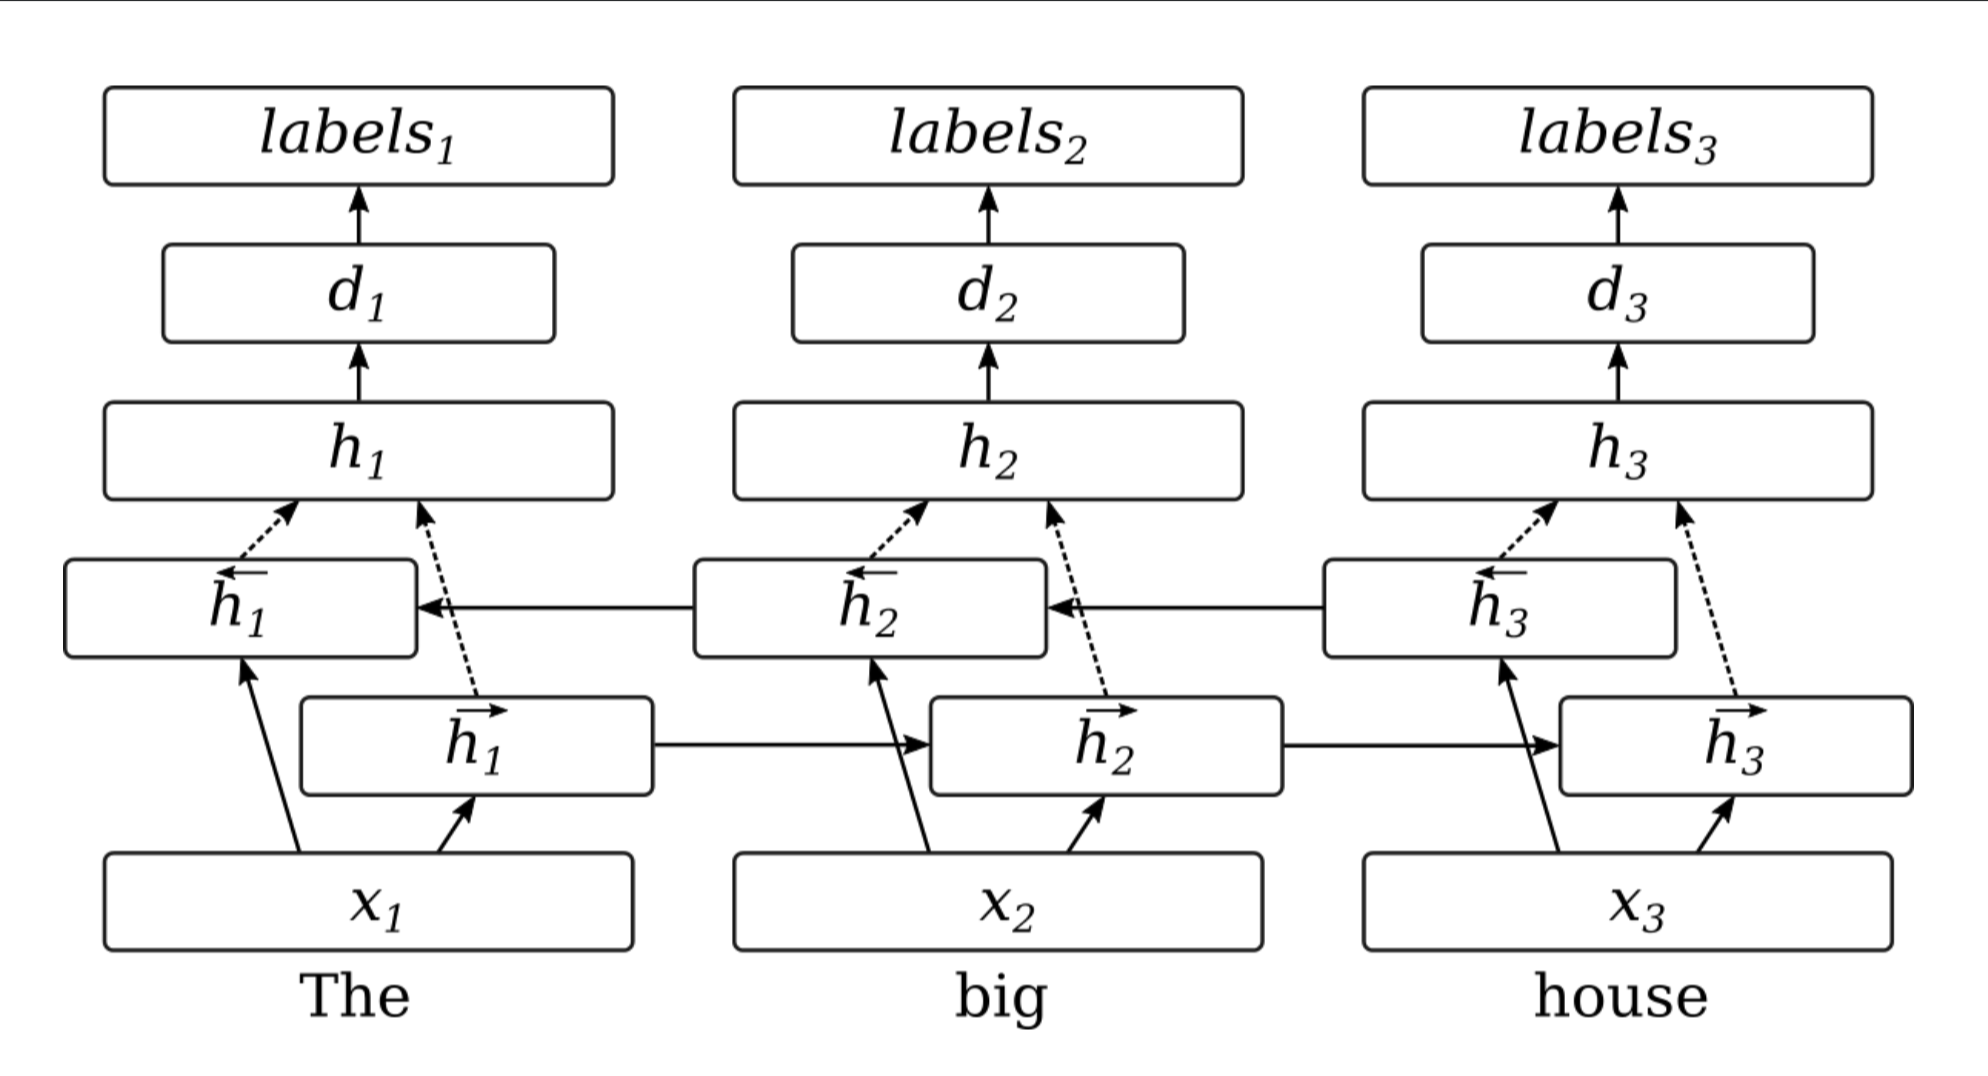
\includegraphics[width=0.7\textwidth]{./__pics/BiLSTM.eps}
	\caption{Схема базовой модели BiLSTM [1]}
\end{figure}

Затем, добавляется скрытый слой нелинейности:
$$d_\text{t} = tanh(W_\text{d}h_\text{t}),$$
где $\textbf{W}_\text{d}$ -- весовая матрица между слоями.

В конце для создания самих меток используется либо softmax либо Conditional Random Fields (разновидность метода Марковских случайных полей) в зависимости от выбранной постановки задачи. Функция softmax рассчитывает нормированное распределение вероятностей по всем возможным меткам для каждого слова:

$$\mathbb{P}(y_t = l| d_t) = \cfrac{e^{W_ld_\text{t}}}{\sum_{\tilde{l}\in K}e^{W_\tilde{l}d_\text{t}}},$$


\paragraph{Усовершенствования базового алгоритма} 

!!! ДЛЯ БУДУЩИХ ТЕСТИРОВАНИЙ
\section{Результаты работы алгоритма}

\paragraph{Базовый алгоритм на датасете MOH}
Тестирование базовой модели BiLSTM привело к результатам в среднем дающим уже после 10 эпох обучения F1-меру $~65\%$
	\begin{figure}[H]
		\centering
		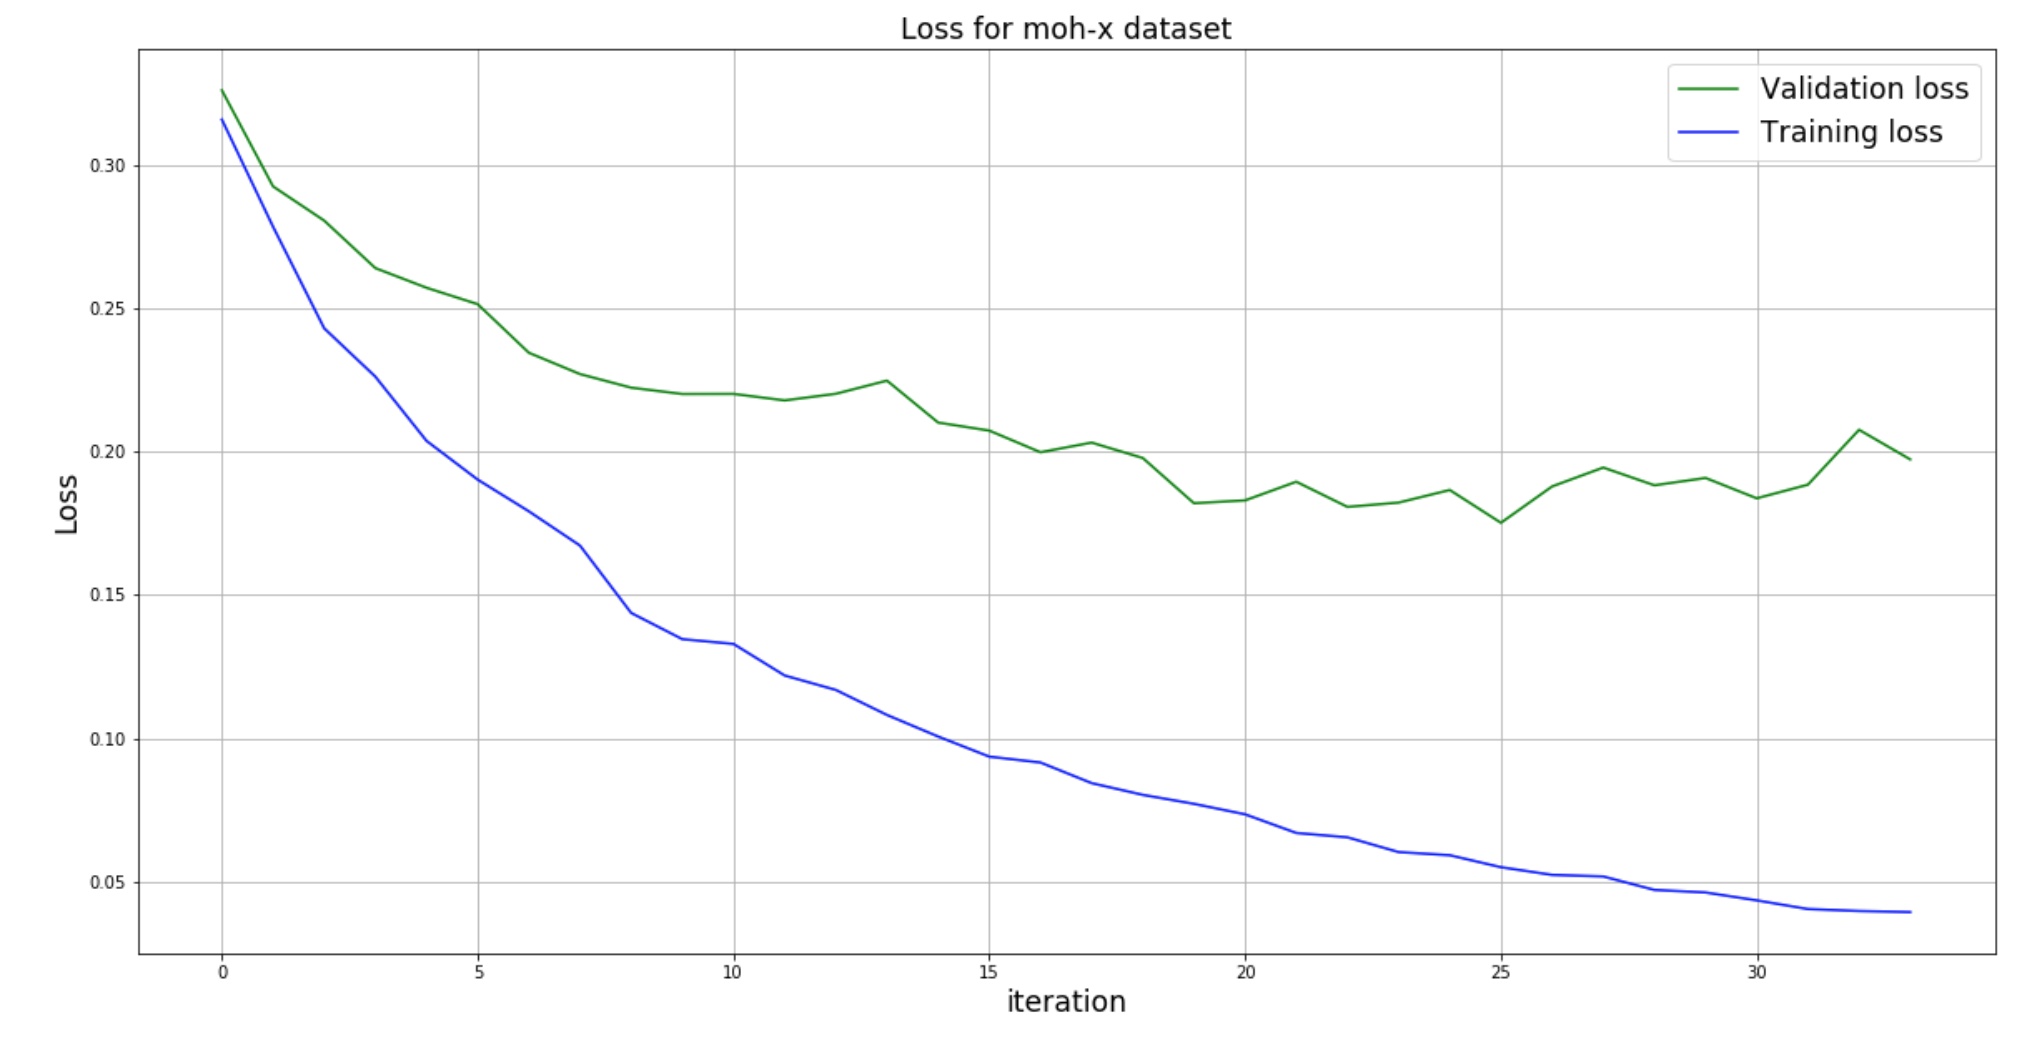
\includegraphics[width=0.9\textwidth]{./__pics/loss.eps}
	%	\caption{Loss на датасете MOH-X}
	\end{figure}
Результаты эксперимента: F1 мера
	\begin{figure}[H]
		\centering
		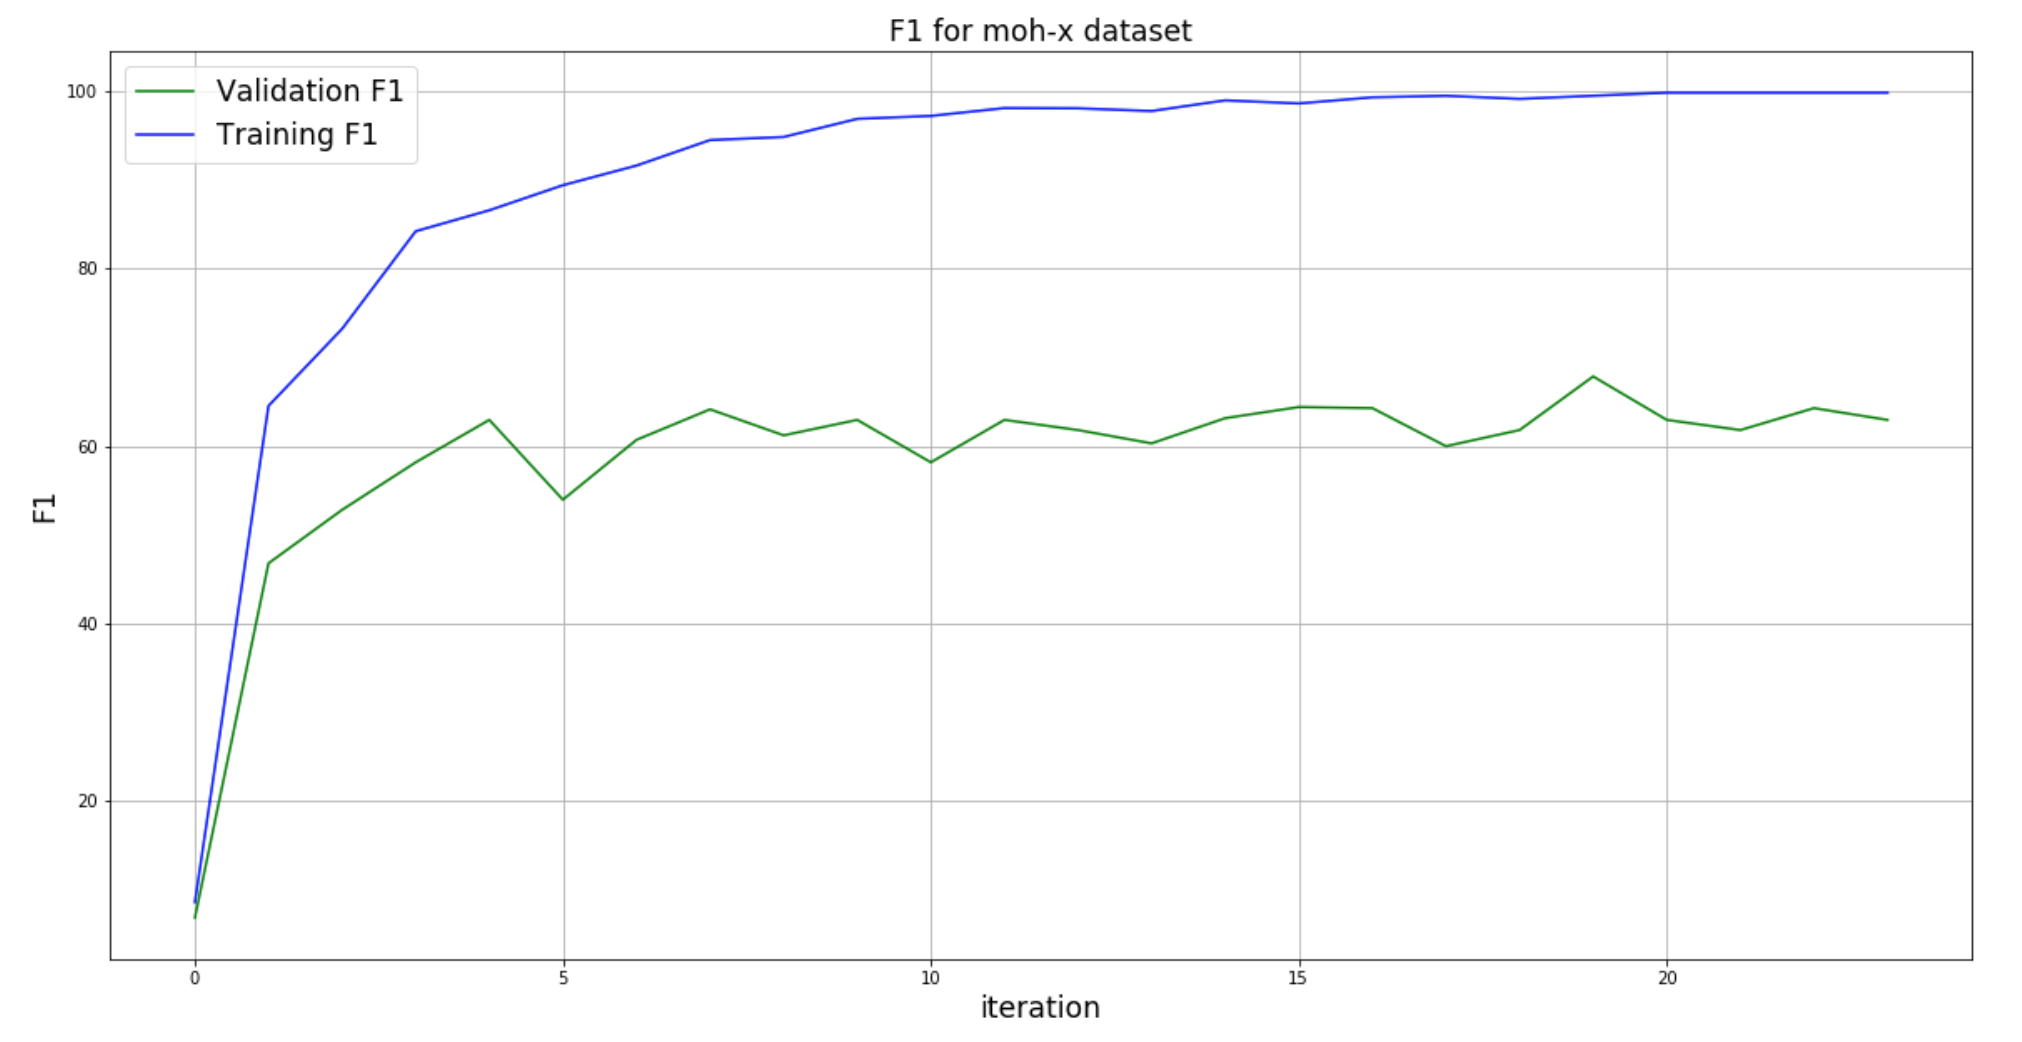
\includegraphics[width=0.9\textwidth]{./__pics/F1.eps}
	\end{figure}
	
			\textbf{	Качество алгоритма после 30 эпох обучения:}
			\begin{itemize}
				\item Precision on MOH =  \textbf{64}.14203612479474
				\item Recall on MOH =  \textbf{67}.85714285714286
				\item F1 on MOH =  \textbf{65}.8939014202172
				\item Accuracy on MOH =  \textbf{69}.27083333333333
			\end{itemize}

\paragraph{Базовый алгоритм на датасете, собранным на русском языке (получен из института русского языка)}
Для датасета "атмосфера". Размер датасета:  2436. Примеров с лэйблом 1: 48.3 \%.
	\begin{figure}[H]
		\centering
		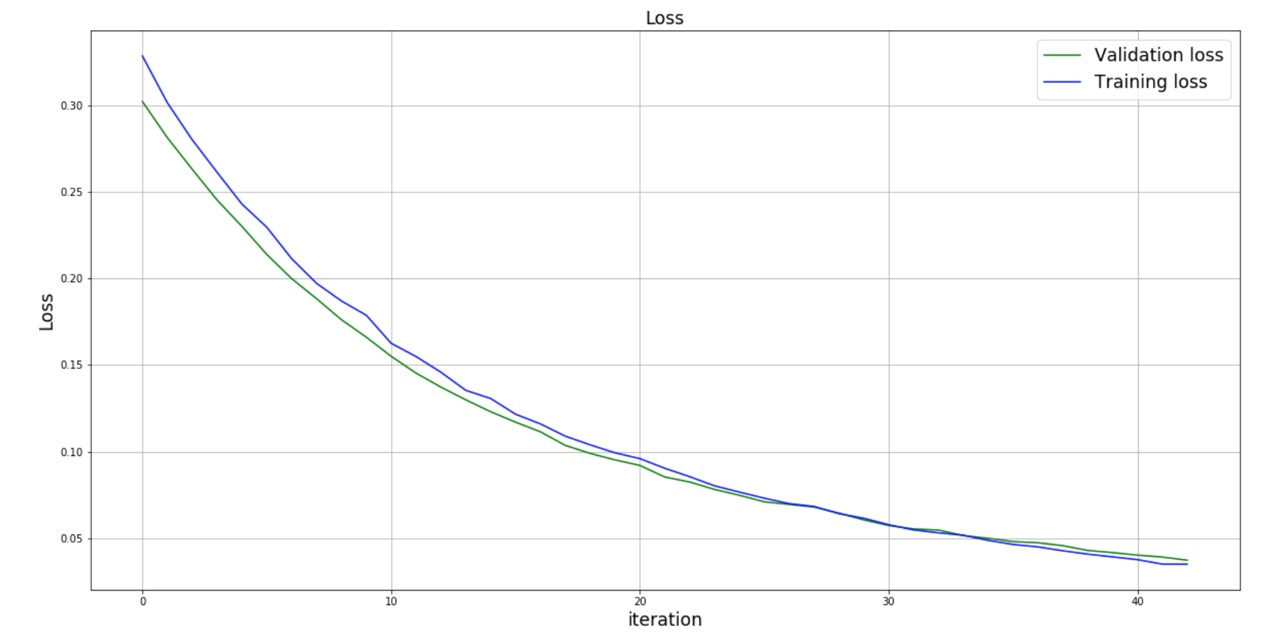
\includegraphics[width=0.9\textwidth]{./__pics/rus_loss}
		%	\caption{Loss на датасете MOH-X}
	\end{figure}
	Результаты эксперимента: F1 мера
	\begin{figure}[H]
		\centering
		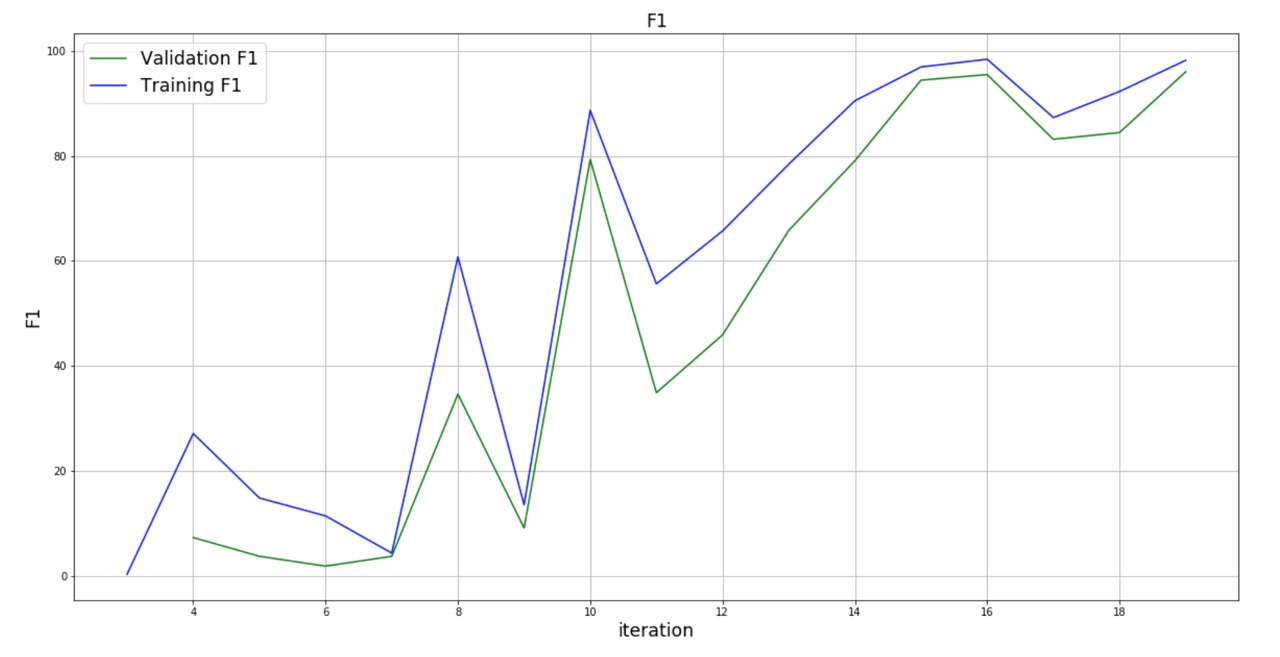
\includegraphics[width=0.9\textwidth]{./__pics/rus_F1}
	\end{figure}
	
	\textbf{Качество алгоритма после 10 эпох обучения:}
	\begin{itemize}
		\item Precision =  \textbf{100}.0
		\item Recall =  \textbf{93}.26923076923077
		\item F1 =  \textbf{96}.51741293532339
		\item Accuracy  =  \textbf{97}.11934156378601
	\end{itemize}

\paragraph{Базовый алгоритм на датасете, основанном на тексте романа М. А. Булгакова "Мастер и Маргарита"}
	
	\textbf{	Качество алгоритма после 10 эпох обучения:}
\begin{itemize}
	\item Precision  =  \textbf{86}.96
	\item Recall  =  \textbf{93}.02
	\item F1  =  \textbf{89}.89
	\item Accuracy  =  \textbf{88}.61
\end{itemize}

%\paragraph{Базовый алгоритм на датасете VUA}
%	Результаты эксперимента: F1 мера
%	\begin{figure}[H]
%		\centering
%		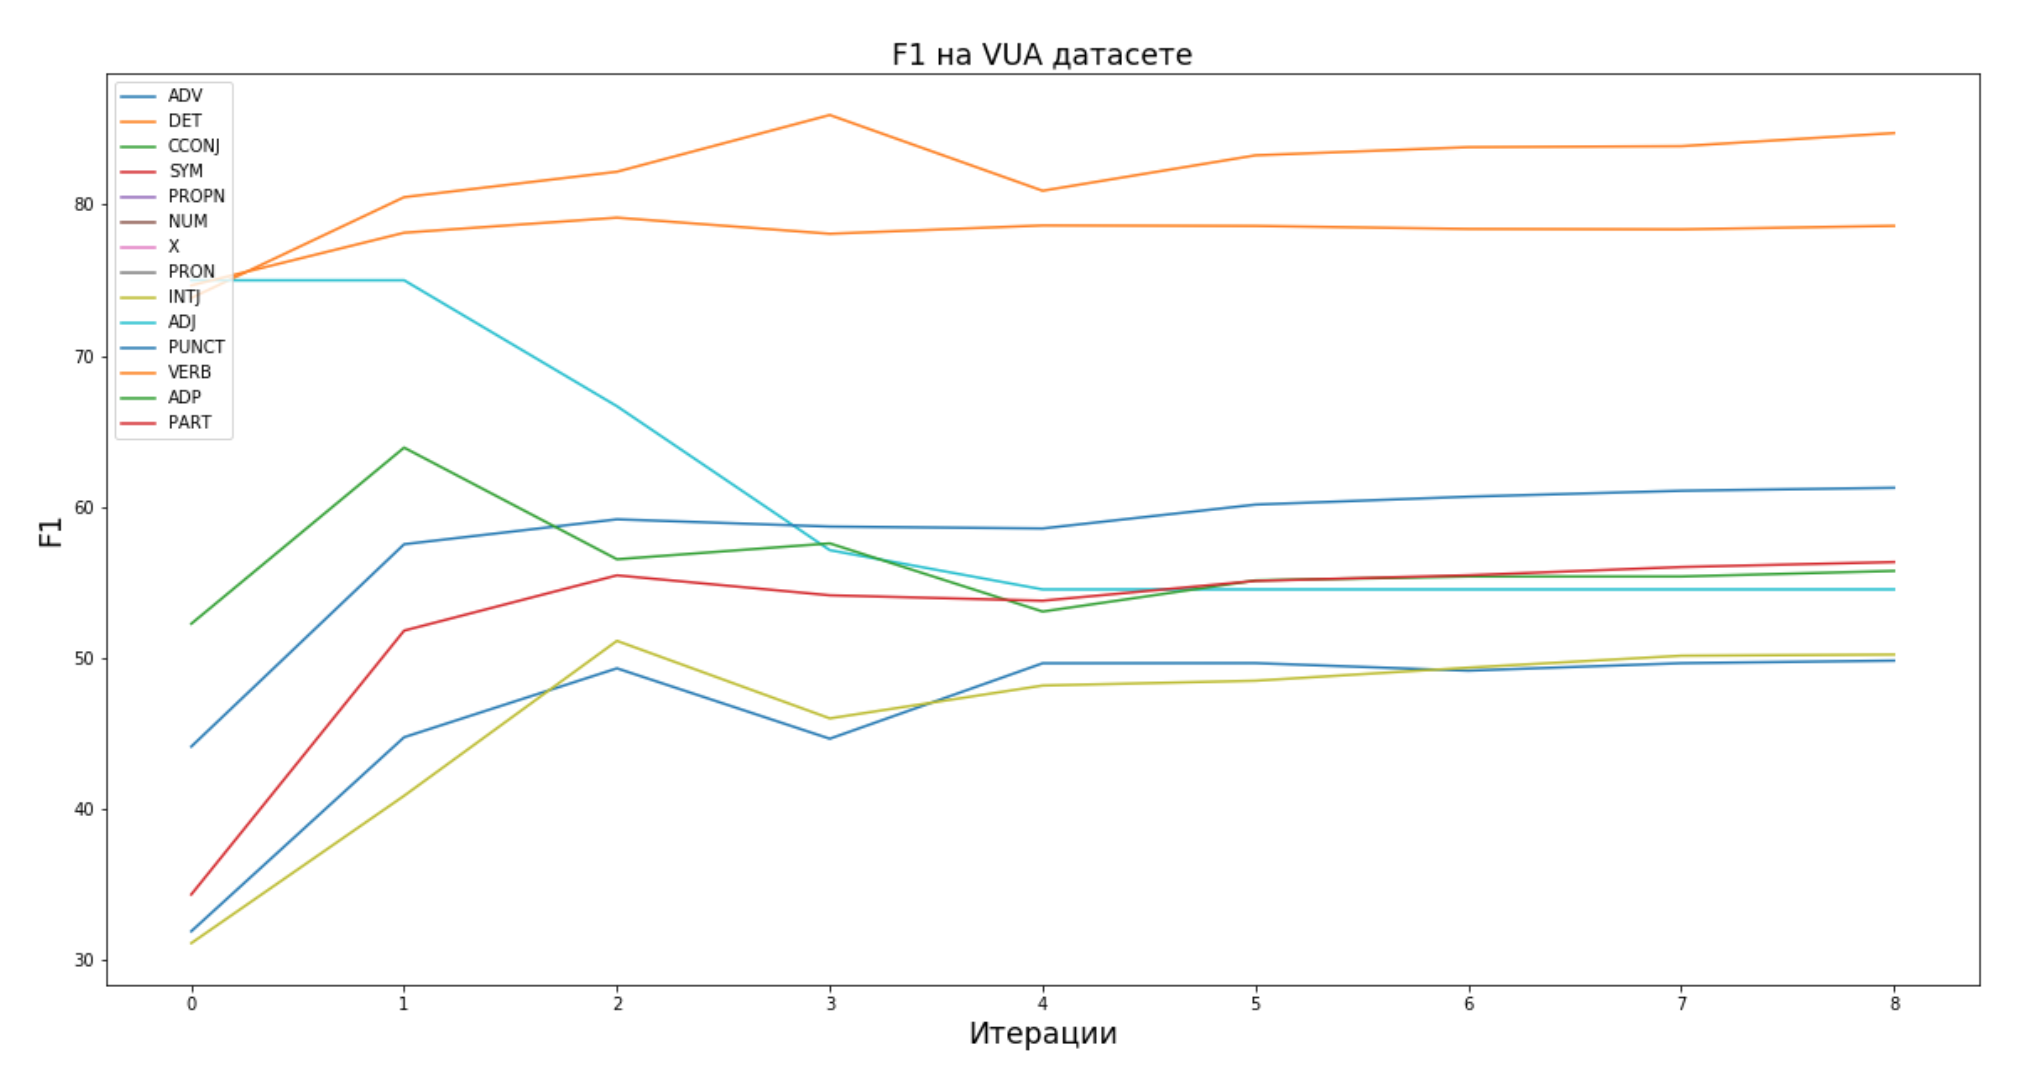
\includegraphics[width=0.9\textwidth]{./__pics/VUA_F1}
%	\end{figure}

\section{Заключение}
	\begin{itemize}
		\item Алгоритм sequence labeling хорошо подходит для поиска символов в тексте
		\item Сравнены результаты работ нескольких моделей: наилучшая – ?
		\item Главная особенность эксперимента -- мало данных
		\item Качество заметно улучшится при увеличении выборки
		\item Для русскоязычных текстов данная задача никак до этого не решалась
	\end{itemize}


\newpage

\begin{thebibliography}{1}

\bibitem{author09anyscience}
    \BibAuthor{Marek Rei, Gamal K.O. Crichton,  Sampo Pyysalo \;N.}
    \BibTitle{Attending to Characters in Neural Sequence Labeling Models}~//
    \BibJournal{Proceedings of COLING 2016, the 26th International Conference on Computational Linguistics: Technical Papers }, 2016, C16-1030, Pp.\,309--318.

\bibitem{author09anyscience}
	\BibAuthor{Adnan Akhundov, Dietrich Trautmann, Georg Groh \;N.}
	\BibTitle{Sequence Labeling: A Practical Approach}~//
	\BibJournal{CoRR }, vol. abs/1808.03926, 2018.

\bibitem{author09anyscience}
	\BibAuthor{Zachary Chase Lipton, John Berkowitz \;N.}
	\BibTitle{A Critical Review of Recurrent Neural Networks for Sequence Learning }~//
	\BibJournal{CoRR }, vol. abs/1506.00019, 2015.

\bibitem{author09anyscience}
	\BibAuthor{Vaswani, Ashish and Shazeer, Noam and Parmar, Niki and Uszkoreit, Jakob and Jones, Llion and Gomez, Aidan N and Kaiser, \L ukasz and Polosukhin, Illia \;N.}
	\BibTitle{Attention is all you need }~//
	\BibJournal{Advances in Neural Information Processing Systems 30}, 2017, Pp.\,5998--6008.

\bibitem{author09anyscience}
	\BibAuthor{Adnan Akhundov, Dietrich Trautmann, Georg Groh \;N.}
	\BibTitle{LONG SHORT-TERM MEMORY}~//
	\BibJournal{Journal Neural Computation archive Volume 9 Issue 8 }, 1997, Pp.\,1735--1780 
%\bibitem{myHandbook}
%    \BibAuthor{Автор\;И.\,О.}
%    Название книги.
%    Город: Издательство, 2009. 314~с.
%\bibitem{author09first-word-of-the-title}
%    \BibAuthor{Автор\;И.\,О.}
%    \BibTitle{Название статьи}~//
%    \BibJournal{Название конференции или сборника},
%    Город:~Изд-во, 2009.  С.\,5--6.
%\bibitem{author-and-co2007}
%    \BibAuthor{Автор\;И.\,О., Соавтор\;И.\,О.}
%    \BibTitle{Название статьи}~//
%    \BibJournal{Название журнала}. 2007. Т.\,38, \No\,5. С.\,54--62.
%\bibitem{bibUsefulUrl}
%    \BibUrl{www.site.ru}~---
%    Название сайта.  2007.
%\bibitem{voron06latex}
%    \BibAuthor{Воронцов~К.\,В.}
%    \LaTeXe\ в~примерах.
%    2006.
%    \BibUrl{http://www.ccas.ru/voron/latex.html}.
%\bibitem{Lvovsky03}
%    \BibAuthor{Львовский~С.\,М.} Набор и вёрстка в пакете~\LaTeX.
%    3-е издание.
%    Москва:~МЦHМО, 2003.  448~с.
\end{thebibliography}

% Решение Программного Комитета:
%\ACCEPTNOTE
%\AMENDNOTE
%\REJECTNOTE
\end{document}
